\documentclass{article}
\usepackage{graphicx}
\usepackage{amsmath}   
\usepackage{amsthm}
\usepackage{tikz}
\usepackage{pgfplots}
\pgfplotsset{compat=1.18}
\usetikzlibrary{pgfplots.polar}
\setlength{\parindent}{0pt}

\title{17-S3-Q5 \\ Solution + Discussion}
\author{David Puerta}
\date{}

\definecolor{BLUE}{RGB}{101,149,179}

\newcommand{\der}[2]{\frac{\mathrm{d}#1}{\mathrm{d}#2}}

\begin{document}

\maketitle

\begin{abstract}
    \noindent In this document we will go through the solution to the 17-S3-Q5 question and provide a discussion of the question at the end. There are also hints on the first page to aid you in finding a solution. There is no single method that results in an answer to a STEP question, there are a multitude of different paths that end up at the same solution. However, some methods are more straight forward and you are encouraged to take the path of least resistance.  
\end{abstract}

\vspace{1cm}

\begin{center}
    \textbf{Hints}
\end{center}

\textbf{First part}: Using the fundamental polar coordinate equations to find $\der{y}{\theta}$ and $\der{x}{\theta}$ then use the chain rule to find $\der{y}{x}$.

\vspace{1cm}

\textbf{Second part}: What is the relationship between the gradients of the curves if they meet at a right angle?

\vspace{1cm}

\textbf{Third part}: Use the relation in the first part to form a differential equation for $\mathrm{f}(\theta)$.

\newpage

\begin{center}
    \textbf{Solution}
\end{center}

Using our fundamental polar coordinate equations
\[
x = \mathrm{f}(\theta) \cos \theta \quad \text{and} \quad y = \mathrm{f}(\theta) \sin \theta 
\]
we can use the chain rule,
\[
\der{y}{x} = \der{y}{\theta} \cdot \der{\theta}{x}
\]
with 
\begin{align*}
    & \der{y}{\theta} = \mathrm{f}'(\theta)\sin\theta + \mathrm{f}(\theta)\cos\theta \\
    & \der{x}{\theta} = \mathrm{f}'(\theta)\cos\theta - \mathrm{f}(\theta)\sin\theta
\end{align*}
to give 
\[
\der{y}{x} = \frac{\mathrm{f}'(\theta)\sin\theta + \mathrm{f}(\theta)\cos\theta}{\mathrm{f}'(\theta)\cos\theta - \mathrm{f}(\theta)\sin\theta} = \frac{\mathrm{f}'(\theta)\tan\theta + \mathrm{f}(\theta)}{\mathrm{f}'(\theta)-\mathrm{f}(\theta)\tan\theta}.
\]

\vspace{0.2cm}

If we have two curves that meet at right angles at a point, then their gradients must also meet at right angles at that same point.\par 
\quad The gradient of the curves $r=\mathrm{f}(\theta)$
\[
m_{\mathrm{f}}= \frac{\mathrm{f}'(\theta)\tan\theta + \mathrm{f}(\theta)}{\mathrm{f}'(\theta)-\mathrm{f}(\theta)\tan\theta}
\]
and $r=\mathrm{g}(\theta)$
\[
m_{\mathrm{g}} = \frac{\mathrm{g}'(\theta)\tan\theta + \mathrm{g}(\theta)}{\mathrm{g}'(\theta)-\mathrm{g}(\theta)\tan\theta}
\]
must have a product of $-1$, 
\[
m_{\mathrm{f}} \ m_{\mathrm{g}}= -1 \ \Rightarrow \ m_{\mathrm{f}}= -\frac{1}{m_{\mathrm{g}}}.
\]
We see that
\[
\frac{\mathrm{f}'(\theta)\tan\theta + \mathrm{f}(\theta)}{\mathrm{f}'(\theta)-\mathrm{f}(\theta)\tan\theta} = 
\frac{\mathrm{g}(\theta)\tan \theta - \mathrm{g}'(\theta)}{\mathrm{g}'(\theta)\tan \theta + \mathrm{g}(\theta)}
\]
gives,
\[
\left(\tan^2\theta + 1\right) \left(\mathrm{f}\mathrm{g} + \mathrm{f}'\mathrm{g}' \right)=0
\]
after some simplification. Thus where they meet we have  $\tan^2 \theta + 1 \equiv \sec^2\theta=0$ which would imply that $\cos \theta =0$, or 
\[
\mathrm{f}(\theta)\mathrm{g}(\theta) + \mathrm{f}'(\theta)\mathrm{g}'(\theta)=0.
\]

\vspace{0.2cm}

Using the above relation with $\mathrm{g}(\theta) = a(1+\sin\theta)$ gives
\[
a\mathrm{f}(\theta)(1+\sin\theta) + a\mathrm{f}'(\theta)\cos\theta=0
\]
for each value of $a$. Solving the differential equation
\[
\der{\mathrm{f}}{\theta} = -\frac{1+\sin\theta}{\cos \theta}\mathrm{f}
\]
involves the integral 
\[
-\int \frac{1+\sin\theta}{\cos \theta}\,\mathrm{d}\theta.
\]
Using the substitution $u = 1+\sin\theta$,
\[
-\int \frac{1+\sin\theta}{\cos \theta}\,\mathrm{d}\theta = -\int \frac{1}{2-u}\,\mathrm{d}u = \ln(1-\sin\theta) + c
\]
and thus we have that 
\[
\ln(\mathrm{f}) = \ln(1-\sin \theta) + c \Rightarrow \mathrm{f}(\theta) = A(1-\sin\theta)
\]
for some $A$. With our initial condition $\mathrm{f}(-\frac{\pi}{2})=4$,
\[
\mathrm{f}(\theta) = 2(1-\sin \theta).
\]

Plotting $r=1+\sin\theta$, $r= 4(1+\sin\theta)$ and $\mathrm{f}(\theta)$,

\begin{figure}[h!]
\centering
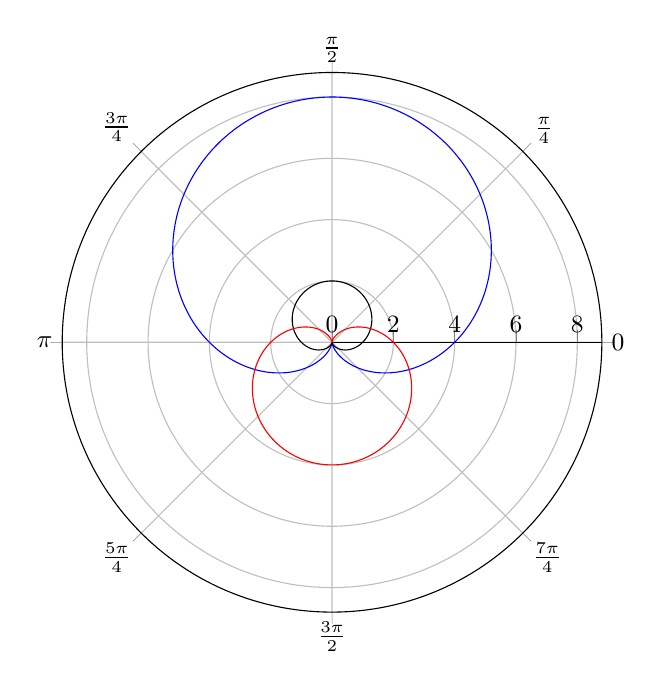
\begin{tikzpicture}
  \begin{polaraxis}[
    xtick={0,45,90,135,180,225,270,315},
    xticklabels={$0$, $\frac{\pi}{4}$, $\frac{\pi}{2}$, $\frac{3\pi}{4}$,
                 $\pi$, $\frac{5\pi}{4}$, $\frac{3\pi}{2}$, $\frac{7\pi}{4}$},
    ticklabel style={font=\small},
    grid=both
  ]
    \addplot[color=blue, domain=0:360, samples=300] {4*(1+sin(x))};
    \addplot[domain=0:360, samples=300] {1+sin(x)};
    \addplot[color=red,domain=0:360, samples=300] {2*(1-sin(x))};
  \end{polaraxis}
\end{tikzpicture}
\end{figure}

with $r=1+\sin\theta$ in black, $r=4(1+\sin\theta)$ in blue and $\mathrm{f}(\theta)$ in red.

\newpage

\begin{center}
    \textbf{Discussion}
\end{center}

\vspace{0.5cm}

Familiarity with the equations of polar coordinates, sketching polar coordinates and Cartesian geometry are key to a understanding of this question.\par
\quad Starting with finding an expression for the Cartesian derivative in terms of $r=\mathrm{f}(\theta)$ and $\theta$ can seem abstract. Writing down the fundamental equations 
\[
x = \mathrm{f}(\theta) \cos \theta \quad \text{and} \quad y = \mathrm{f}(\theta) \sin \theta 
\]
and the chain rule
\[
\der{y}{x} = \der{y}{\theta} \cdot \der{\theta}{x}
\]
helps clarify what we know and what we need. The rest is differentiation and algebraic manipulation. \par
\quad Showing the relation 
\[
\mathrm{f}(\theta)\mathrm{g}(\theta) + \mathrm{f}'(\theta)\mathrm{g}'(\theta)=0
\]
is conceptually the easiest if we consider the relation of the Cartesian form of the curves $r=\mathrm{f}(\theta)$ and $r=\mathrm{g}(\theta)$ as in this form we are comfortable with the fact that their gradients must have a product of $-1$.\par
\quad Substituting our given curves leads to a standard separable differential equation which can be solved to find $\mathrm{f}(\theta)$.\par
\quad To sketch a polar curve it is typically a good rule of thumb to recognise the standard curves (lines and circles in polar coordinates) in combination with finding the values of $\theta$ where $\der{r}{\theta}=0$, $r=0$ and values of $r$ for certain theta (such as $\theta=0,\frac{\pi}{6},\frac{\pi}{4},\frac{\pi}{3},\cdots$).\par
\quad Overall, proficiency with polar coordinates and sketching polar curves will lead to a smooth experience in tackling this question. 


\end{document}
